\documentclass[border=5pt,multi=page]{standalone}
\usepackage{tikz}
\usetikzlibrary{arrows.meta}
\definecolor{diagramInk}{HTML}{184052}
\definecolor{diagramFill}{HTML}{EDF5F7}
\tikzset{paper box/.style={draw=diagramInk!75,fill=diagramFill,
  rounded corners=2pt,align=center,inner sep=4pt,font=\sffamily\scriptsize},
  paper arrow/.style={-{Stealth[length=4pt]},draw=diagramInk,thick}}
\begin{document}
\begin{page}
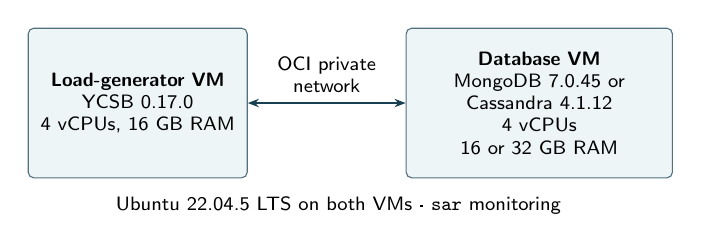
\begin{tikzpicture}
\node[paper box,text width=25mm,minimum height=19mm] (load) at (0,0)
  {\textbf{Load-generator VM}\\YCSB 0.17.0\\4 vCPUs, 16 GB RAM};
\node[paper box,text width=31mm,minimum height=19mm] (db) at (51mm,0)
  {\textbf{Database VM}\\MongoDB 7.0.45 or\\Cassandra 4.1.12\\4 vCPUs\\16 or 32 GB RAM};
\draw[{Stealth[length=4pt]}-{Stealth[length=4pt]},draw=diagramInk,thick]
  (load.east) -- node[above,align=center,font=\sffamily\scriptsize] {OCI private\\network} (db.west);
\node[below=2pt,font=\sffamily\scriptsize,align=center] at (25.5mm,-10mm)
  {Ubuntu 22.04.5 LTS on both VMs · \texttt{sar} monitoring};
\end{tikzpicture}
\end{page}
\begin{page}
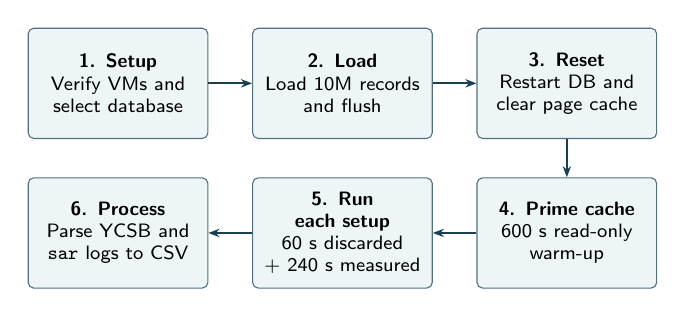
\begin{tikzpicture}[stepbox/.style={paper box,text width=20mm,minimum height=14mm}]
\node[stepbox] (pre) at (0,0) {\textbf{1. Setup}\\Verify VMs and\\select database};
\node[stepbox] (load) at (28.5mm,0) {\textbf{2. Load}\\Load 10M records\\and flush};
\node[stepbox] (reset) at (57mm,0) {\textbf{3. Reset}\\Restart DB and\\clear page cache};
\node[stepbox] (warm) at (57mm,-19mm) {\textbf{4. Prime cache}\\600 s read-only\\warm-up};
\node[stepbox] (run) at (28.5mm,-19mm) {\textbf{5. Run each setup}\\60 s discarded\\+ 240 s measured};
\node[stepbox] (parse) at (0,-19mm) {\textbf{6. Process}\\Parse YCSB and\\\texttt{sar} logs to CSV};
\draw[paper arrow] (pre) -- (load);
\draw[paper arrow] (load) -- (reset);
\draw[paper arrow] (reset) -- (warm);
\draw[paper arrow] (warm) -- (run);
\draw[paper arrow] (run) -- (parse);
\end{tikzpicture}
\end{page}
\end{document}
